\section{Key Management in Space DTNs}
\label{sec:survey}

A Key management system has fundamental goals: secrecy of keys and assurance of purpose \cite{martineveryday}.  DTNs present fundamental differences with traditional networks that make goals of protocols sometimes unclear or difficukt to define, and key management is not the exception. Cryptographic key management is considered one of the most challenging problems in DTNs \cite{menesidou2016automated,menesidou2017cryptographic,ivancic2009security,asokan2007towards}. This section focuses on the study of the problem, defines a set of requirements to evaluate the solutions, and presents a survey of proposed key management systems for space DTNs.


\subsection{Current Key Management Systems}


The first question that arises is whether symmetric or asymmetric keys should be used in key management. The section \ref{sec:space} concludes that symmetric keys are the most suitable option for current space missions, but future space missions will present an entirely new scenario.

For the Interplanetary Internet a scenario similar to the terrestrial Internet is expected \cite{rationale2010requirements}. Multi-hop communication and cross-organisational domains are enhancements on current interplanetary communications. Also, policies, rights, hierarchy, and administrative groups will form part of future deep space networks. The system might scale to thousands of nodes, and different organisations will participate in the network. Therefore, a key management system similar to the Internet, like TLS certificates, seems more suitable. 

The research effort so far is based on some form of public key management. Templin \cite{templin-dtnskmps-00} states the need for delay tolerant automated systems for distribution of authenticated public keys and revocations mechanism, which are not available yet. Although there are ciphersuites based on symmetric keys in the BSP \cite{ietf-dtn-bpsec-07}, there is a common consensus that public key management will be the preferred method for the Interplanetary Internet. 

%Furthermore, symmetric keys might not be even acceptable in a cross-organisational domain \cite{ivancic2009security}. 

In public key management based on certificates,  nodes must have a copy of the destination public key to encrypt the message, and the destination node must have the sender public key to verify integrity. Key distribution is not a sensitive operation in the sense that the information is not secret.  Common techniques to obtain public keys are \textbf{pushing} directly from the key owner and \textbf{pulling} from a (usually) trusted directory \cite{martineveryday}.

Relatively low delays on the Internet allows pushing and pulling to be effective to retrieve public keys. For instance, a TLS handshake uses the pushing approach to get the destination certificate. After obtaining the certificate, the node needs to check its validity with a Certificate Authority (CA). Popular options for this validation process are certificate revocation list (CRL) or the Online Certificate Status Protocol (OCSP), but these options require interaction with the CA which might not be available in deep space communications. 

%There are modifications of OCSP to improve the message overhead, but these are designed to alleviate the overhead on certificates receivers, but the overhead is transferred to the other side of the communication. In Secure/Multi-purpose Internet Mail Extensions (S/MIME) sender could encapsulate its certificate as meta-data, but the receiver is expected to validate the information. S/MIME remove the communication between nodes but still require on-demands interactions with a trusted authority. 

There are other alternatives to public key management based on certificates. Templin \cite{templin-dtnskmps-00} consider that web of trust might be an option for some types of DTNs, but argue that more research should be done. For space-based networks, a model without a trusted authority is not acceptable \cite{viswanathan-dtn-pkdn-00,burleigh-dtnwg-dtka-01,ivancic2009security}.  

Another alternative widely explored is based on Identity Based Cryptography ID-PKC. This approach eliminates the requirement of public certificates, and in consequence, some problems inherent to the management of certificates, but it introduces others issues such as key escrow and key revocation. These problems can be addressed but no without adding considerably overhead which questioned the benefits of ID-PKC for DTNs. In any case, proposal based on ID-PKC are considered in this work.


%Another alternative widely explored is based on Identity Based Cryptography ID-PKC. This approach uses a direct derivation of the public key from the node ID and eliminates the requirement of public certificates.  Even though IBC eliminates some problems inherent to the management of public certificates, it introduces other issues such as key escrow and key revocation. These problems can be addressed but no without adding considerably overhead which questioned the benefits of IBC for DTNs.


  


\subsection{Taxonomy of key Management in DTNs}
\label{sec:taxonomy}

% Creo que ya esta repetido.
Key management includes a wide range of processes which together provide security to cryptographic keys.  The problem of secure administration of cryptographic keys is complex but well-understood on terrestrial networks. Future space-based networks present two challenges to key management systems. Firstly, the network topology is dynamic; it consists of heterogeneous space nodes and planned communication links, opportunistic links might be available as well. Secondly, traditional cryptographic protocols are not suitable for this type of network; this problem is widely discussed in previous sections.


Menesidou \textit{et al.} \cite{menesidou2017cryptographic} classify key management schemes into three categories depending on whether the system deals or not with secure initialisation, key establishment, and revocation. Key establishment is divided again into two groups: two-party and group communication. The same classification is adopted in this work. 

%As this project aims to choose the most suitable key management scheme for the Interplanetary Internet, assumptions and benefits are scrutinised. 

A space DTN has the same goals as terrestrial networks for key management, but the hostile environment demands extra considerations. Researchers interpret these extra considerations in different ways. For instance, some of them argue that public certificates are not suitable because this model requires queries to a central authority which may be inaccessible. In consequence, some propose ID-PKC, others propose decentralised and fully distributed models.  

%Many of these schemes adopted different metrics and requirements. Thus, it seems that the problem is not well understood and the it is not requirements are not clear. 


One objective of this project is to analyse the key management systems so far proposed and conclude which model suit best for the Interplanetary Internet. For that purpose, a set of requirements must be defined beforehand. This work considers most of the requirements proposed by Templin  \cite{templin-dtnskmreq-00} plus a scalability requirement. The omitted requirements defined by Templin are discussed later in section \ref{sec:evaluation}. It is worth to mention that these requirements complement the fundamental requirements for a key management system, and do not replace them. 

The following list enumerates the set of requirements (REQ) define in this work.

\begin{enumerate}
    \item Keys must be available when needed. The design must not rely on a query-response interaction between a source node and the trusted party or a destination node. This implies that credentials must be cached ``locally''. DTN nodes must store the information or the access to them must be subject to low delay and rarely disrupted links.
    \item The system must be trustworthy. There must be a trust anchor in the system for all operations; for instance nodes cannot accept information directly from other nodes without a previous trust.
    \item A single point of failure is not acceptable. Nodes cannot depend only on the access to one entity,  some type of high availability must be present in the system.
    \item The system must support secure bootstrapping of nodes. The association between a node ID and its credentials (key or administrative information) must be certified before a node can use it.
    \item The system must support delay tolerant key revocation. The system must have the capability to revoke keys before the expiry date. 
    \item The systems must be scalable. A space DTN could grow to thousands of nodes and the system must be capable of dealing with this situation. 
    \item The system must be compatible with the Bundle Protocol and the Bundle Security Protocol.
\end{enumerate}

Two desirable characteristics related to the performance are defined. First, the key management system should impose minimal latency in addition to the physical delay. Second, the key management system should not impose more than a reasonable amount of messages and storage overhead. Extreme conditions in the space make these characteristic difficult to achieve; the solution has to give up some efficiency to solve the problem under the imposed constraints, specifically storage overhead. Mission planners will prefer a system with low overhead given that it satisfies the fundamental requirements. Finally, it is desirable if the key management system does not need to modify the current specifications of the Bundle Protocol. 
  

The REQ 1 encompasses the fundamental problem for DTN nodes, which is the access to authenticated information without online interaction with a CA, distribution centre or other nodes. In conclusion, the availability of authenticated information is the central problem for a key management system. 


\subsection{A Survey of Key Management for Space DTNs}

This work evaluates various key management system according to the requirements defined before. The analysis considers protocols which focus only on key distribution because this problem is critical for key management, as stated previously.

Seth and Keshav \cite{seth2005practical} propose a solution for general disconnected environments. They argue that disconnected nodes cannot efficiently use a certificate infrastructure because this requires queries to a central database, and certificates revocations list are not suitable for the excessive delay. This work uses Hierarchical IBC for creating secure channels providing mutual authentication and key revocation to some degree. There is one Private Key Generator (PKG) per domain which administrates the registration and establishment of system parameters. This requires the exchange of several messages, but this procedure is done only once. The authors proposed USB key storage devices to distribute symmetric keys from PKG to final users prior deployment. For revocation, they used time-based keys where the PKG updates periodically every node with a new time-stamped private key. Cross-domain communication requires an online look-up of the destination system parameters. The proposal fails to meet the same requirements of key revocation, secure bootstrapping and single point of failure.

Another solution based on ID-PKC is proposed by Aniket \textit{et al.} \cite{kate2007anonymity}. This solution is more efficient than the previous one because a source node does not need to look up the public parameters of DTN nodes in different domains. Instead, nodes can use the root PKG parameters to communicate with nodes in other domains. They also use a single-flow non-interactive key agreement scheme to exchange symmetric keys. This system also fails to meet the same requirements as the previous solution. However, the authors suggest a secret sharing scheme instead of using a single PKG to avoid a single point of failure. This paper is the only one that provides an anonymity architecture, but this requires updating the domain PKG's master key, and the renewal of all users private keys periodically. CCSDS \cite{book2011space} does not consider anonymity as a requirement for space DTNs. In any case, the Bundle in Bundle Encapsulation \cite{ietf-dtn-bibect-00} already provides a way to achieve anonymity. 

Xie and Wang \cite{xie2013practical} propose a different approach based on bilinear pairing. The method uses a self-certified identity scheme and a distributed key generation that requires only an initial broadcast message rather than multiple interactions. Prior deployment, users obtain a digital ID card granted by a relevant authority and the system parameters. Then, each node generates its private key and distributes an initial message containing its credentials. When a node receives the initial message, it needs to verify if the signature matches with the credentials, then compute a secret sharing and extract the encryption parameters. Unlike the previous schemes, this provides secure bootstrapping, but revocation is not supported. Others problems are that the system is not scalable and new DTN nodes receive information directly from other nodes.

Van Vesien \cite{van2010dynamic} presents a non-interactive key distribution using bilinear maps over elliptic curves. This work is one of the few that explains in detail how the key exchange protocol fits with the BSP specification. For instance,  the protocol could be used to exchange keys for HMAC-SHA 1 authentication, RSA digital signature, and AES encryption. Each node is a member of one or more groups, and only nodes in the same group can non-interactively exchange keys. Initially, a group administrator calculates a value for each node using a master key and the node ID.  Then the administrator provides the calculated value to each node before deployment. Two hosts can non-interactively establish a shared secret given the value provided by the group administrator, and the bundle parameters. This proposal only focuses on key distribution, and there are no mentions of initialisation or revocation. Scalability might be an issue because in practice a node can only be a member of two groups.


%For solving the key management problem, Jadhav \textbf{et al.} proposed using a time-evolving topology model and two channel cryptography to design a non-interactive key exchange protocol. This protocol assumes two channel, one insecure and one secure usually called Out-Of-Band OOB channel. The first stage is the bootstrap where the key owner present directly to the authority the authentication information and this could be easily checked. 

Lv \textit{et al.} \cite{lv2014non} present another non-interactive key establishment solution for space DTNs. The protocol uses a time-evolving model to exchange information such as keys or revocation status, and two-channel message authentication. In the bootstrapping stage, DTN nodes authenticate with a CA via an Out-of-Band (OOB) channel providing secure initialisation. The OOB channel involves human interaction such as space missions authorities. In the exchange phase, a node sends its public key over an insecure channel like a radio signal to another node, then it calculates the hash of the public key and sends over the OOB channel. The receiver has to verify that the public key has not been modified. The authors suggest a laser emitter and a photo-sensor, but they state that the design of an OOB channel is an open issue for space networks.  Another problem is that key distribution and revocation are performed without the intervention of the authority.  

%Even if the development of laser technology is a promising technology for communication in space, it is unlikely that this will  Besides, there is no need to use the insecure channel if a secure OOB optical channel is available.

Butha \textit{et al.} \cite{bhutta2014efficient} present a key transport protocol to exchange symmetric keys which are compliant with the BSP. The system uses a proxy signatures scheme which does not require a secure channel. This scheme provides hop-by-hop authentication for the Bundle Authentication Block BAB. Each intermediate node validates the bundle, remove the BAB, and generates a new BAB using proxy signatures. The issue with this scheme is that the last version on the BSP eliminated the BAB because detecting the next security-aware node is difficult or impossible to achieve in some situations contemplated by the BP, so the overhead added by proxy signatures is not justifiable. This solution does not address at all problems like initialisation or revocation.

Andrade and Pessoa \cite{de2016fully} propose a fully distributed public key management using digital signatures chains for DTNs. The system does not present a single point of failure and works in the presence of intermittent connectivity. In fixed intervals, nodes send the list of chains identifying the origin of each chain. A receiving node re-signs the chain and sends to other nodes if the verification is correct. A chain is open if a node was able to verify all signatures until the origin, otherwise, it is a closed chain. The system does present a trust anchor for operations, but the system is able to resist several attack to the infrastructure. Key revocation is not supported.


The most recent proposal is an IETF Internet-Draft  The Delay-Tolerant Key Administration DTKA is a system of public key management for space-based DTNs. This Internet-draft \cite{burleigh-dtnwg-dtka-01}, released in 2018, is a full specification for the entire life-cycle of public keys. The system adopts the publisher/subscriber model to proactively distribute public keys from the Key Agents (KA) to Key Users. One or more KAs share the key authority role. DTN nodes register with the Key Authority through an OOB channel (for instance a physical channel). The Key Agents generate bulletins with authenticated information such as new or revoked certificates and distribute the bulletins using a t-n threshold scheme. Finally, nodes reassemble the bulletins and update their local database. All information in the bulletin is for future use, so nodes do not depend on immediate access to bulletins. Scalability might be an issue for the DTKA. This solution is further discusses at the end of this section.  

R\"{u}sch \textit{et al.}  \cite{rusch2017forward} argue that in traditional PKC and ID-PKC secret keys are valid for months and the exposure of the secret key allows the decryption of all communications since its creation. They propose puncturable encryption for highly asynchronous scenarios to provide forward secrecy. Their scheme ensures forward secrecy of messages at the cost of higher latency. Nodes may repeatedly update their decryption key to revoke decryption capabilities for some recipients, time intervals, or messages without exchanging new keys.  The authors assumed that a public infrastructure for key exchange and revocation exists,  but they use forward secure encryption keys instead of traditional public keys. There is no mention of initialisation or distribution in this work.



Butta \textit{et al.} propose a scheme based on NOVOMODO \cite{micali2008efficient} to reduce the size of revocation list in DTNs. The new validation and revocation mechanism complies with the Bundle Protocol and X.509 certificates. This work does not deal with initialisation or distribution, and they assume that exists an infrastructure that registers and distributes certificates. The scheme reduces the size of certificates and arranges CRL in form of has tables to increase the efficiency.



Group key management is the base for multicast communication and group-oriented applications \cite{jiang2008survey}. This project does not focus on group communication, but a summary of some works is presented. Group key management can be classified into centralised, decentralised and distributed. The critical security requirements for group key management are forward secrecy, backward secrecy, collusion freedom and key independence \cite{camtepe2005key}. Nodes could join or leave the group, and efficiency and security are desirable in these operations.


Xu \textit{et al.} \cite{xu2012chinese} propose a group key management mechanism based on the Chinese Remainder Theorem for space DTNs. The advantages are that the system does not need to broadcast messages when a node joins the domain, and only send one message when a node leaves the domain. This work uses a stateless scheme to overcome delays and high error rates. For many to many communication they add a lifetime to the group key, this is to deal with users leaving the group.  If a node does not receive the key update message at the determined interval, it can direct inquiry to a neighbour reducing the latency, but this is unacceptable for space-based networks.

Another approach is proposed by Zhou \textit{et al.} \cite{zhou2014autonomic} based on one-encryption multi-decryption key protocol for deep space. Authors claim that their scheme is more efficient than previous ones, but nodes could perform the join and leave operation without the authority. They argue that the operation has the property of forward-security and backward-security if the key independence condition holds.

In group key management, groups are dynamic: authorised member are allowed to join the group and an administrator could expel members from the group. From the requirements defined in this section and reports by CCSDS \cite{standard2010ccsds,book2012architecture,book2006security} it is clear that a centralised approach suit best to space-based networks. It is expected that nodes rarely join or leave a domain, and when this happens, the operation could be done in advance. It still remain more work on this topic. 

Recently, Menesidou and Vasilios \cite{menesidou2016automated} studied the problem of key management on opportunistic DTNs. They argue that key management is better exploited when used in conjunction with routing decision by security-aware nodes. They used the critical path method (CPM) where the duration of each activity is the end-to-end delay and the critical path represent the path with longest delay. The idea is that security aware nodes can exploit the slack time to perform key management operations. The authors developed a protocol parser for evaluating complex scenarios in space DTN.


Table \ref{table:summary} presents a summary of all key management solutions study in this work, it shows whether the proposals deal or not with the most challenging parts: initialisation, distribution, and revocation. It shows as well if each solution is for two-party or group distribution and the method or scheme used.  

Table \ref{table:summaryREQ} shows which requirements satisfies each solution for two-party communication. Note that an ``x'' mark appears in the case the system does not meet the requirement or does not address the problem at all.    

%The table illustrated the proposals and the part of the problem that these schemes address, specifically, registration, establishment and update/revocation. 

\begin{landscape}

\begin{table}[hbt]
\begin{tabular}{lccccc}
 & \multicolumn{5}{l}{\cellcolor[HTML]{000000}{\color[HTML]{EFEFEF} Classification of key management systems}} \\
Ref. & \multicolumn{1}{l}{\cellcolor[HTML]{C0C0C0}Init/Reg} & \multicolumn{1}{l}{\cellcolor[HTML]{C0C0C0}Dist.} & \multicolumn{1}{l}{\cellcolor[HTML]{C0C0C0}Rev.} & \multicolumn{1}{l}{\cellcolor[HTML]{C0C0C0}Individual/Group} & \multicolumn{1}{l}{\cellcolor[HTML]{C0C0C0}\centering Method} \\
\cellcolor[HTML]{C0C0C0}Seth and Keshav\cite{seth2005practical}  & $\surd$ & $\surd$ &  & indiv & HIBC, HIBE and HIBS \\
\cellcolor[HTML]{C0C0C0}Aniket \textit{et al.}\cite{kate2007anonymity} & $\surd$ & $\surd$ &  & indiv & HIBC \\
\cellcolor[HTML]{C0C0C0}Xie and Wang\cite{xie2013practical} & $\surd$ & $\surd$ &  & indiv & distributed secret generation, bilinear pairing, self-certify identity \\
\cellcolor[HTML]{C0C0C0}Van Vesien \cite{van2010dynamic} & & $\surd$ &  & indiv & IBC bilinear maps over elliptic curves \\
\cellcolor[HTML]{C0C0C0}Lv \textit{et al.} \cite{lv2014non} & $\surd$ & $\surd$ &  & indiv &  time evolving model, two-channel cryptography \\
\cellcolor[HTML]{C0C0C0}Butha \textit{et al.} \cite{bhutta2014efficient} &  & $\surd$ &  & indiv & certificates, proxy signatures \\
\cellcolor[HTML]{C0C0C0}Andrade and Pessoa \cite{de2016fully}  & $\surd$ & $\surd$ &  & indiv & decentralised, PGP, signatures chains \\
\cellcolor[HTML]{C0C0C0}Burleigh \textit{et al.}\cite{burleigh-dtnwg-dtka-01} & $\surd$ & $\surd$ & $\surd$ & indiv & certificates, bulletins \\
\cellcolor[HTML]{C0C0C0}R\"{u}sch \textit{et al.}\cite{rusch2017forward} &  &  & & indiv & puncturable encryption, forward secure keys \\
\cellcolor[HTML]{C0C0C0}Butha \textit{et al.} \cite{bhutta2016public} &  &  & $\surd$ & indiv & certificates, CRL, hash tables \\
\cellcolor[HTML]{C0C0C0}Xu \textit{et al.} \cite{xu2012chinese} & $\surd$  & $\surd$ & $\surd$ & group & chinese theorem remainder \\
\cellcolor[HTML]{C0C0C0}Zhou \textit{et al.} \cite{zhou2014autonomic} & $\surd$ & $\surd$ & $\surd$ & group & logical key hierarchy , one-encryption multiple-decryption keys \\ \end{tabular}
\caption{Summary of key management systems}
\label{table:summary}
\end{table}

\end{landscape}


\begin{table}[hbt]
\begin{tabular}{@{}lccccccc@{}}
 & \multicolumn{7}{l}{\cellcolor[HTML]{000000}{\color[HTML]{EFEFEF} key Management Requirement}} \\
 Ref. & \multicolumn{1}{l}{\cellcolor[HTML]{C0C0C0}REQ 1} & \multicolumn{1}{l}{\cellcolor[HTML]{C0C0C0}REQ 2} & \multicolumn{1}{l}{\cellcolor[HTML]{C0C0C0}REQ 3} & \multicolumn{1}{l}{\cellcolor[HTML]{C0C0C0}REQ 4} & \multicolumn{1}{l}{\cellcolor[HTML]{C0C0C0}REQ 5} & \multicolumn{1}{l}{\cellcolor[HTML]{C0C0C0}REQ 6} & \multicolumn{1}{l}{\cellcolor[HTML]{C0C0C0}REQ 7} \\
\cellcolor[HTML]{C0C0C0}Seth and Keshav \cite{seth2005practical}  &  & $\surd$ &  & $\surd$ &  &  & $\surd$ \\
\cellcolor[HTML]{C0C0C0}AniKet \textit{et al.} \cite{kate2007anonymity} & $\surd$ & $\surd$ &   &   &  &  & $\surd$ \\
\cellcolor[HTML]{C0C0C0}Xie and Wang \cite{xie2013practical} & $\surd$ & & $\surd$  & $\surd$  & &  & $\surd$ \\
\cellcolor[HTML]{C0C0C0}Van Vesien \cite{van2010dynamic}  & & $\surd$ & & $\surd$  & & & $\surd$ \\
\cellcolor[HTML]{C0C0C0}Lv \textit{et al.} \cite{lv2014non} & $\surd$ &  &  & $\surd$  &  &  & $\surd$ \\
\cellcolor[HTML]{C0C0C0}Butha \textit{et al.} \cite{bhutta2014efficient} & $\surd$ & & &  & & $\surd$ & $\surd$ \\
\cellcolor[HTML]{C0C0C0}Andrade and Pessoa \cite{de2016fully} & $\surd$ &  & $\surd$  &  & & $\surd$ & $\surd$ \\
\cellcolor[HTML]{C0C0C0}Burleigh \textit{et al.} \cite{burleigh-dtnwg-dtka-01}   & $\surd$   & $\surd$   & $\surd$ & $\surd$ & $\surd$  &  & $\surd$  \\
\cellcolor[HTML]{C0C0C0}R{u}sch \textit{et al.}\cite{rusch2017forward}   & $\surd$  & $\surd$ &  & $\surd$ &  &  &   \\
\end{tabular}
\caption{Key Management Systems VS Requirements}
\label{table:summaryREQ}
\end{table}






\subsubsection{Delay Tolerant Key Administration}

The previous analysis shows that no key management solution satisfies all requirements. The Delay Tolerant Key Administration (DTKA) draft is the most complete solution, it includes all problematic parts of the life-cycle, achieves almost all requirements, and proposes a fault tolerance distribution scheme. Besides, it clearly defines the entities involved in the system and their interaction, the initialisation phase, key distribution, key update, and revocation. A detailed description of the system is presented below.  

The architectural elements (DTKA Entities) are:

\begin{itemize}
  \item  Key Agent (KA) is a node part of the trust anchor of the system. Many KAs collaborate to perform the Key Authority role. Together, KAs construct bulletins with authenticated information and distribute them among subscriber nodes.
  \item Key Owner (KO) is a node with the private key corresponding to the public key authenticated by the Key Authority.
  \item Key User (KU) is a node that receives bulletins from KAs and distribute the information within a single machine.
\end{itemize}

There are others architectural elements define in the DTKA but their interaction in the system is out-of-scope of the document, so these entities are not considered in this work. In practice, most of the DTN nodes will take KO and KU roles.


Figure \ref{fig:dtka} shows the interaction between entities and the assumption. Key Agents must be interconnected using sub-second one-way-light-time (OWLT) and rarely disrupted links. This requirement restricts the deployment of KAs on a terrestrial network, connected probably by the Internet. A time synchronization mechanism (TSM) is required as well by Key Agents such as NTP. A potentially delayed and disrupted channel interconnects KAs with the rest of the DTN, generally the space segment of the DTN. In the space segment, nodes have an own source of clock with an allowed drift of a few seconds.     


\begin{figure}[htb]
\centering
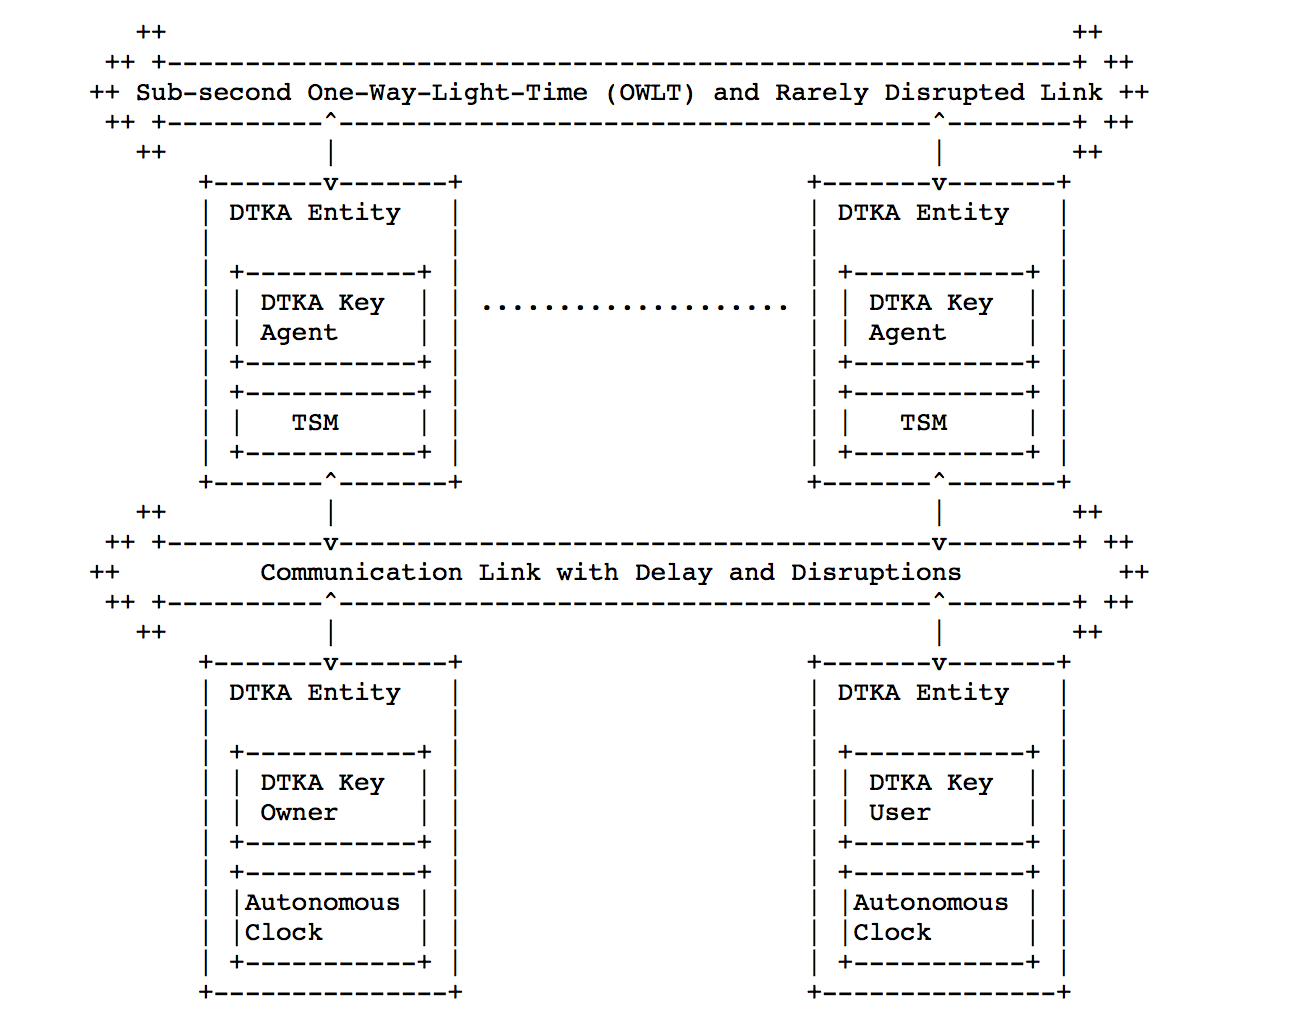
\includegraphics[width=1 \linewidth]{images/DTKA.png} 
\caption{DTKA System interactions, extracted from \cite{burleigh-dtnwg-dtka-01}}
\label{fig:dtka}
\end{figure}

Each KO has a unique endpoint ID and generates its private-public pair. For registration, KOs send an association message via an OOB physical channel signed with its private key.  The signature is only to prove that the node is in possession of the private key corresponding to the public key. Registration requires a manual check of the message received via the physical channel by the Key Authority. Note that KOs have to send registration messages to all KAs in one application domain, producing a demanding operational overhead

Nodes can periodically renew their public-private key pairs following the ``key roll-over protocol''. The roll-over protocol is similar to the registration process but does not require the OOB channel and the current private key is used to sign the association request. Like the registration request, this request must be sent to all KAs, see Figure \ref{fig:Node registration}.

\begin{figure}[htb]
\centering
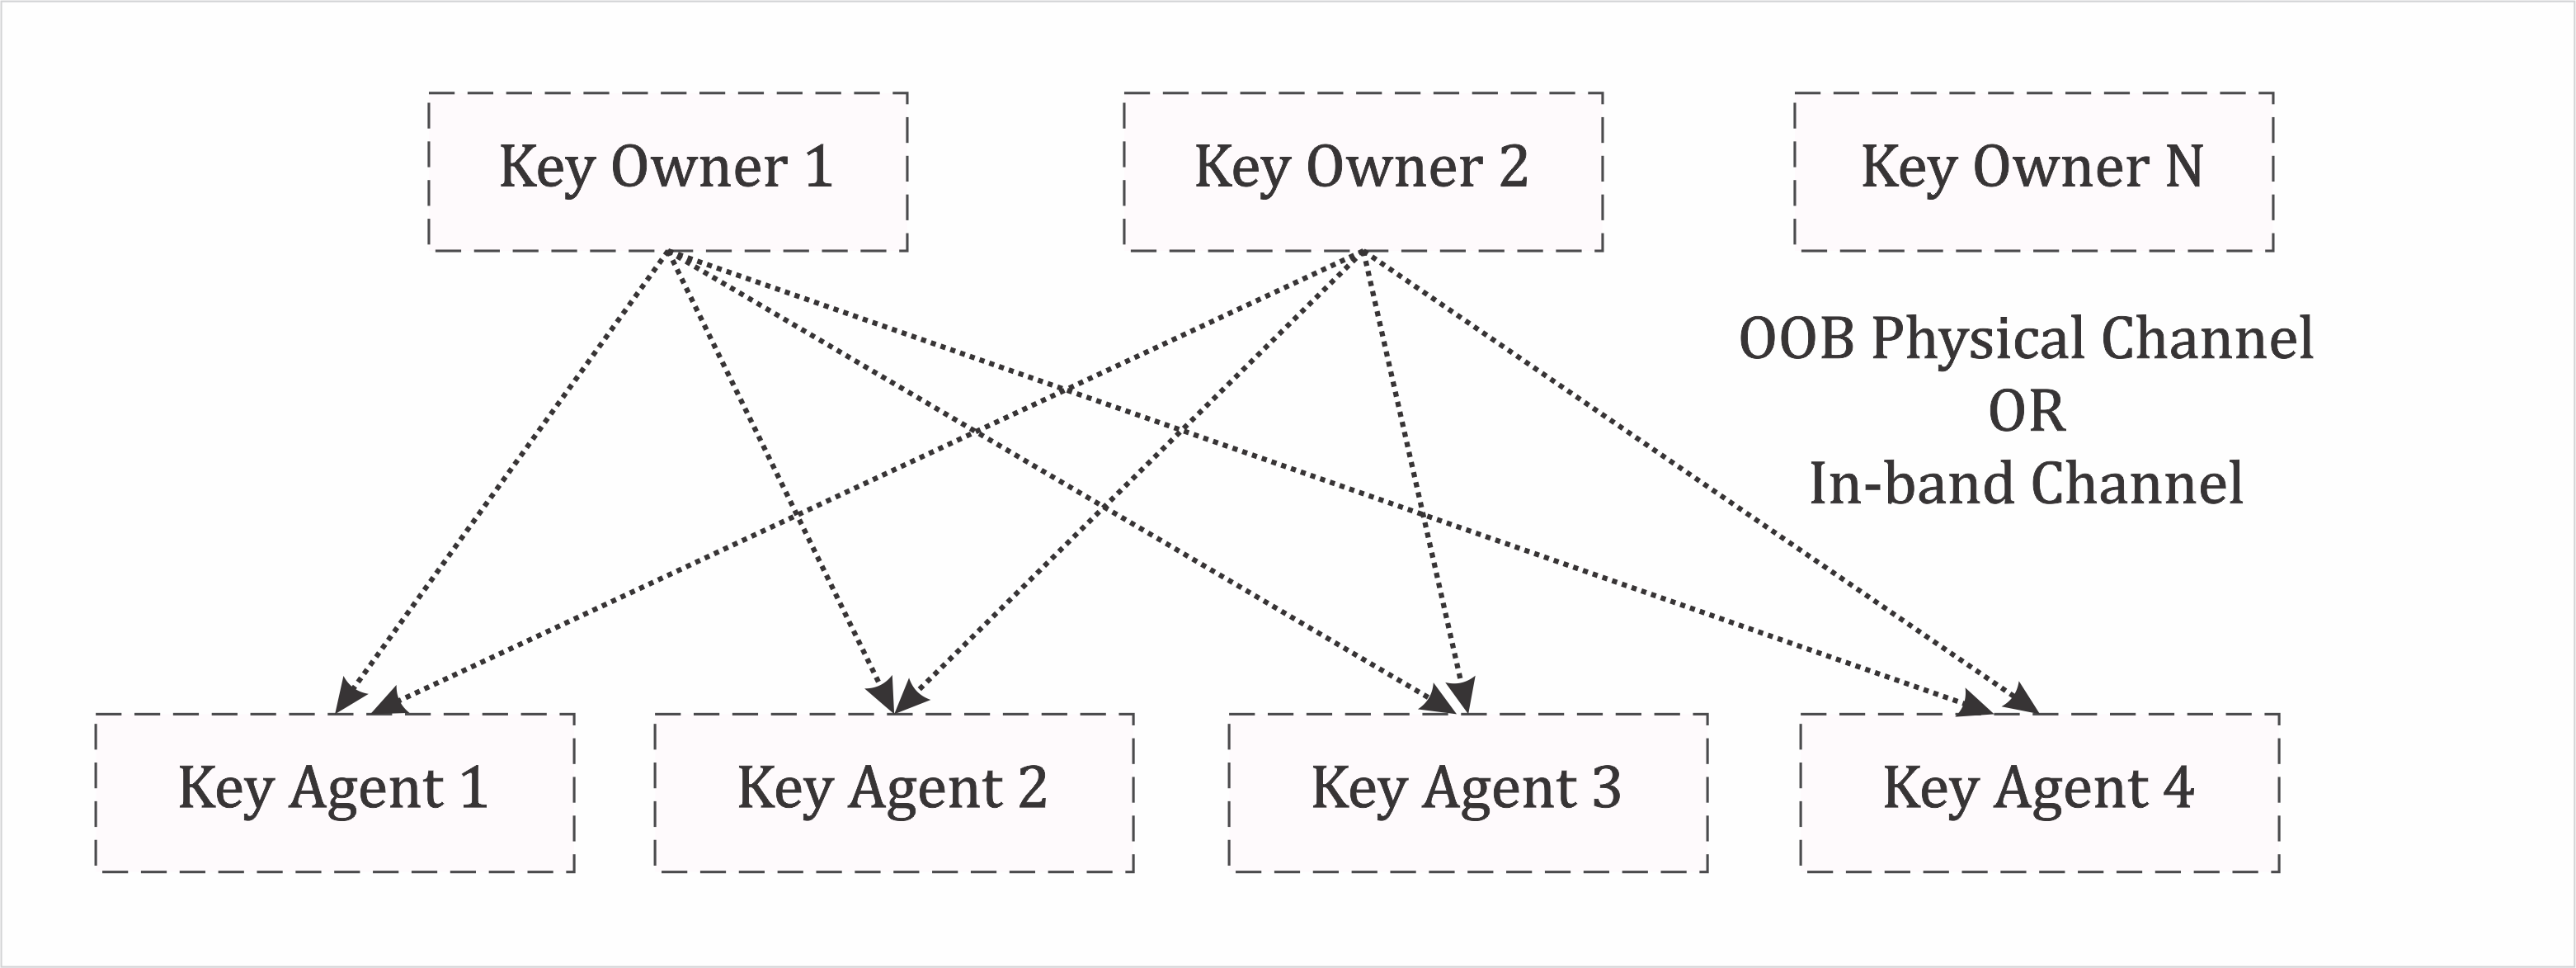
\includegraphics[width=1 \linewidth]{images/node-regist.png} 
\caption{Node registration}
\label{fig:Node registration}
\end{figure}

An association block contains a single association or revocation pair  \textless ID , public key \textgreater. A bulletin is a collection of association blocks. Each bulletin contains an unique sequential identifier (serial number), and a trust model value. For instance, a list of KAs designated to multicast parts of the bulletin and a t-out-n threshold.

The revocation procedure requires a human operator to initiate the process. The operator authenticates to the respective KA, identify the public key, and instruct a schedule revocation message. The KA then send out the message to all other KA instructing to include the revocation message in the next bulletin.   


Key Agents collect multiple association and revocation request from different parties; then they reach consensus on a subset of the requests (Figure \ref{fig:consensus}). Finally, a hash is computed over the subset of association blocks. Once the bulletin is complete, a (Q+R)-erasure code algorithm is used to encode the content, and the output is divided into multiple code blocks. 

\begin{figure}[htb]
\centering
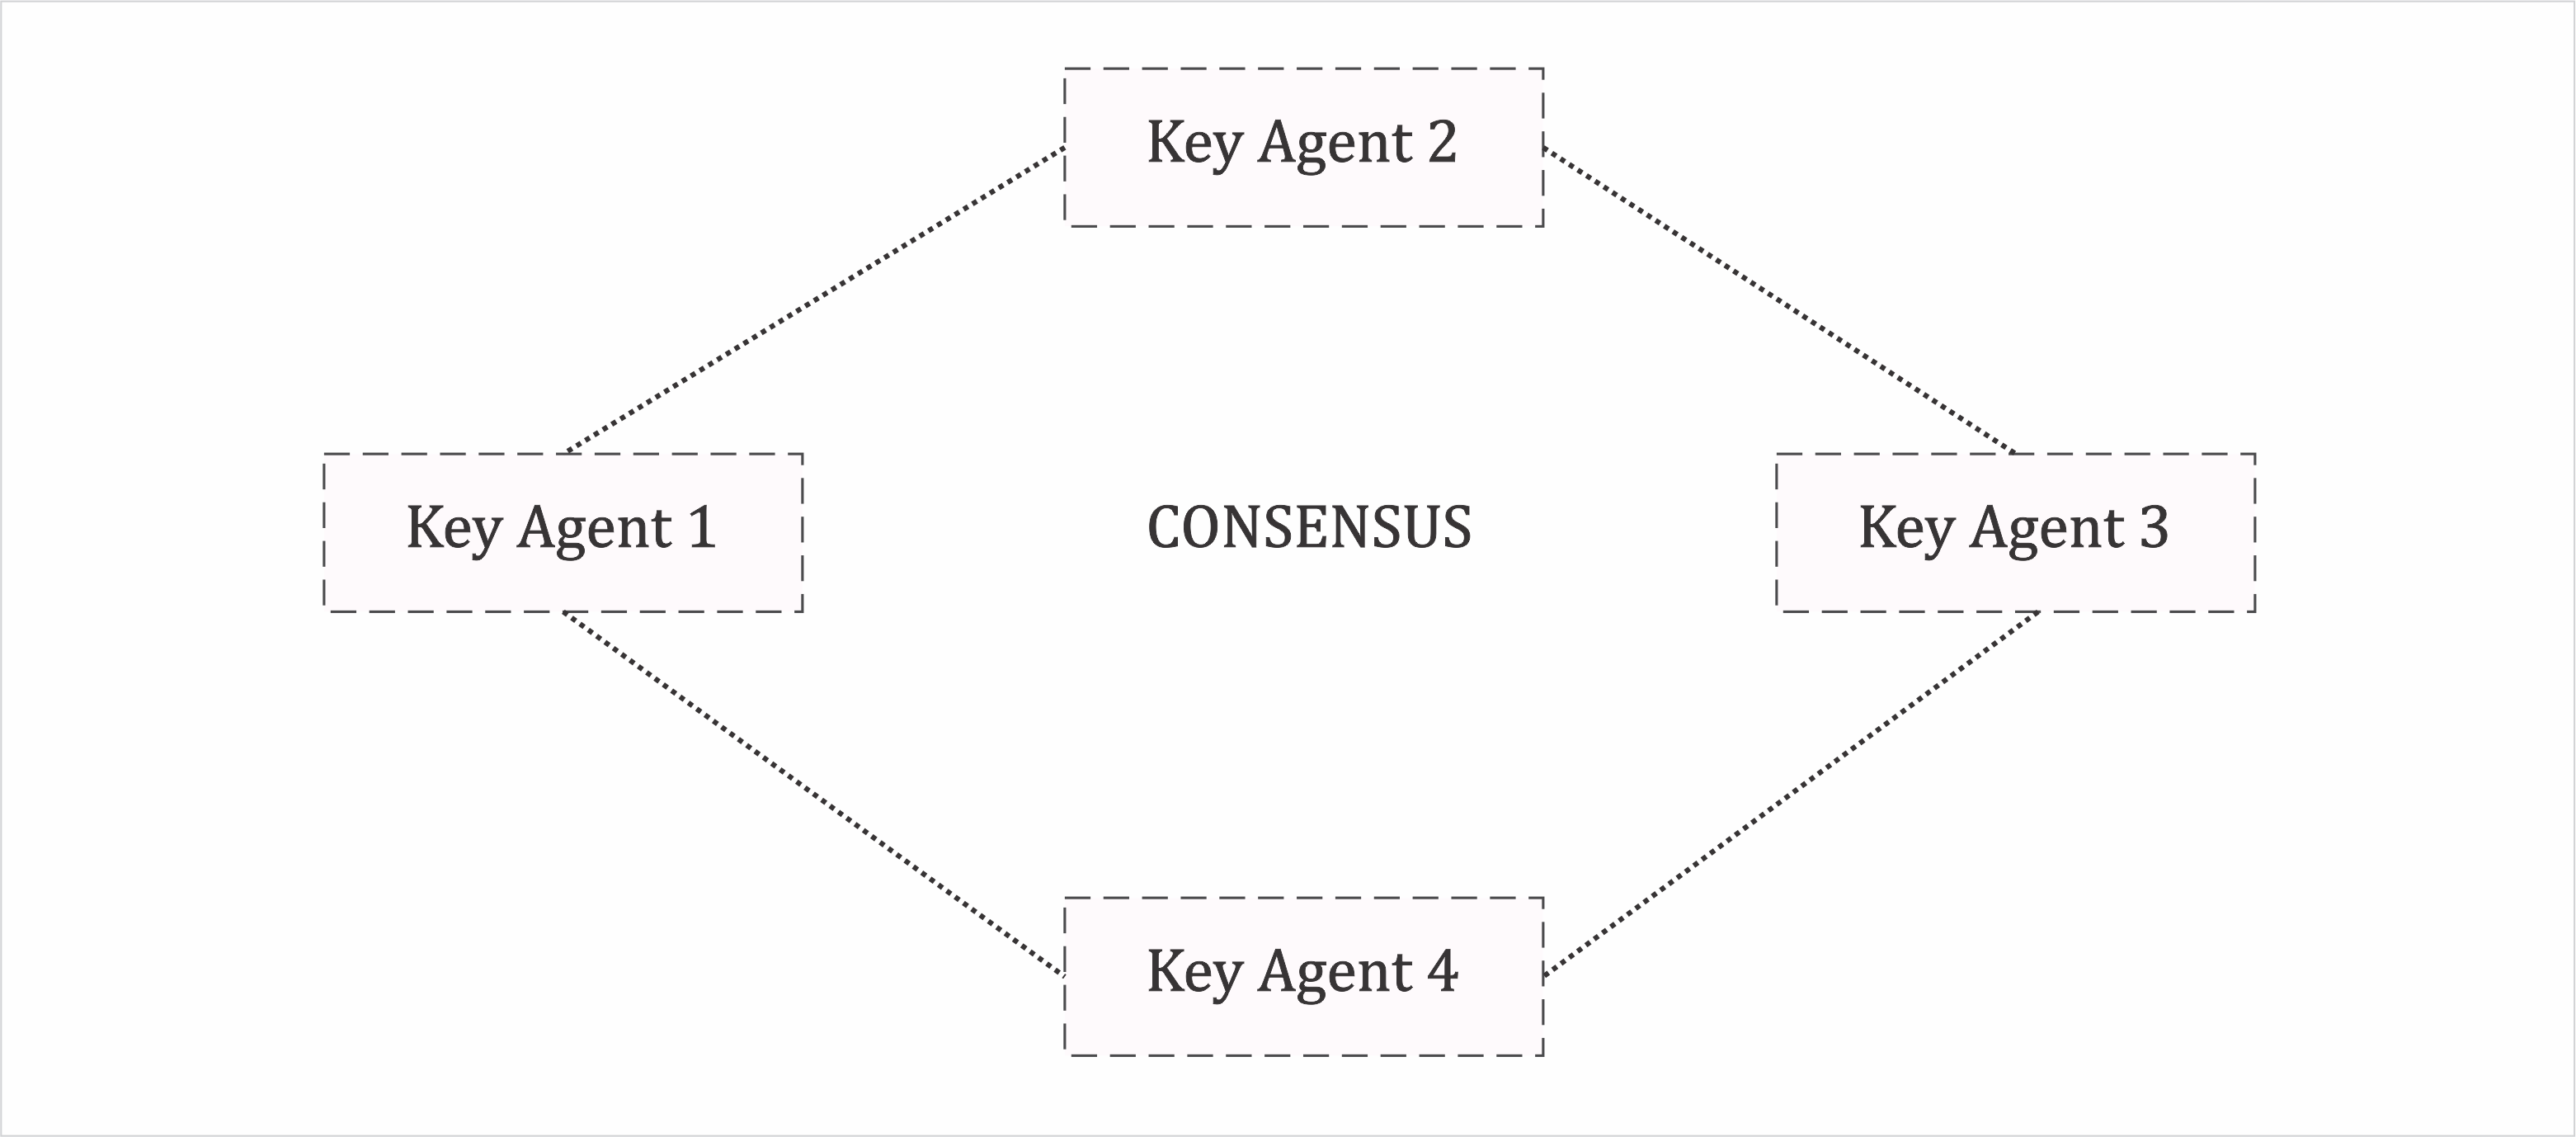
\includegraphics[width=1 \linewidth]{images/consensus.png} 
\caption{Key Authority consensus}
\label{fig:consensus}
\end{figure}


Each KA is responsible for the distribution of a subset of code blocks and has the backup responsibility for others. When a KU receives a code block, it has to verify the authenticity of the message. After accepting some code blocks (t-out-n threshold), the KUs can decode the bulletin and store the information locally. Other defense mechanisms are used to deal with compromised KAs. The reader is referred to \cite{burleigh-dtnwg-dtka-01} for further details.


In summary, bulletin distribution (Figure \ref{fig:distribution}) supports message authentication to avoid spurious messages and redundancy to ensure that a minimal set of KAs multicast the information. The distribution protocol minimises the likelihood of clients being unable to decode the bulletin. The bulletin itself does not contain any signature because each code block is the payload of a bundle protected with a Block Integrity Block of the BSP.

\begin{figure}[hb]
\centering
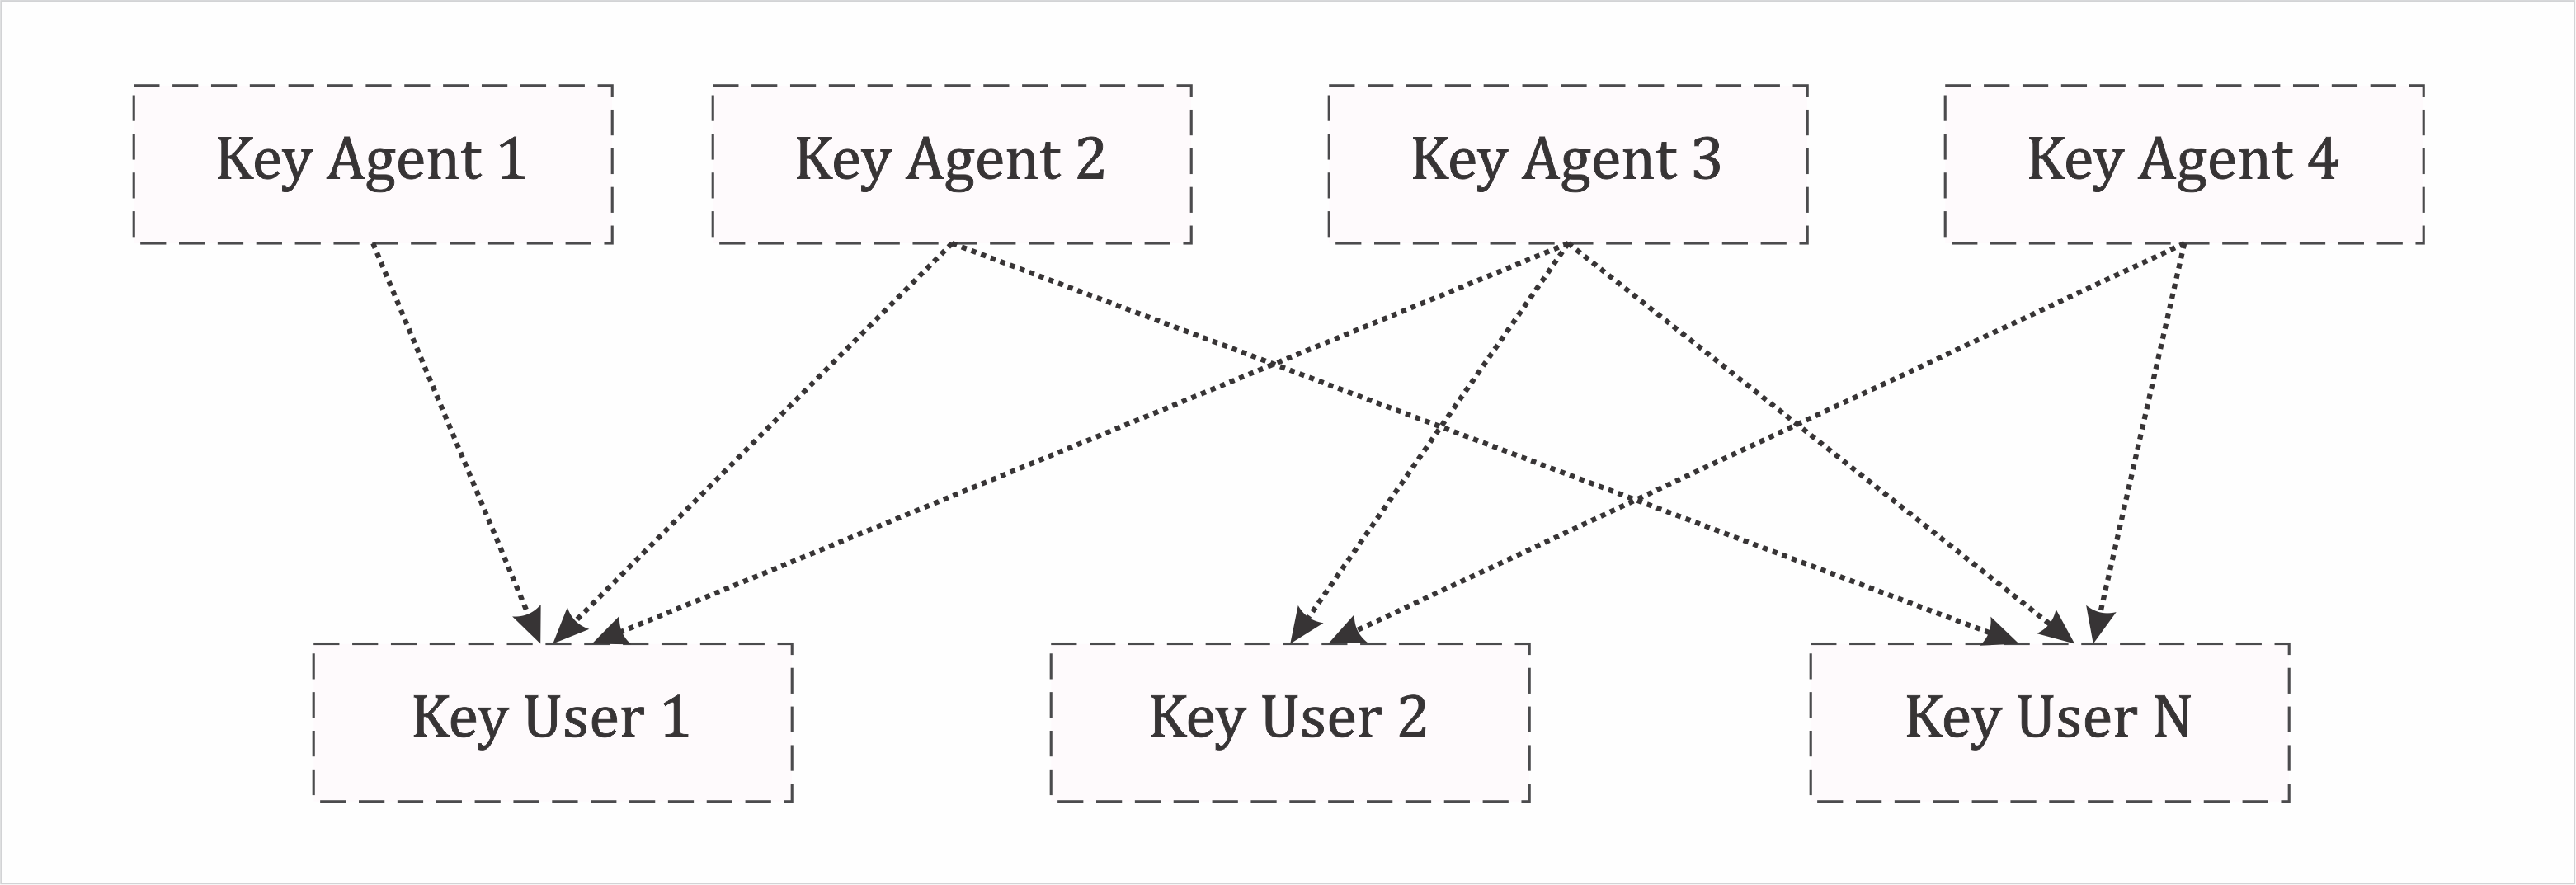
\includegraphics[width=1 \linewidth]{images/distribution.png} 
\caption{Bulletin distribution}
\label{fig:distribution}
\end{figure}

\subsubsection{Issues with DTKA }


A potential problem occurs when an application domain has many KAs. In this case, KOs have to send association requests to all KAs via the OOB physical channel. It is important to consider two aspects of this process. First, a KO is a bundle node and not a physical node such as a spacecraft, which could contain many bundle nodes, potentially thousands. Second, KAs will be geographically distributed to guarantee availability.

This strong registration mechanism is proper for critical space nodes such as relay satellites or space stations, but for light-wave nodes like robots or sensor, it seems an overwhelming overhead which mission planners may not be keen on tolerating. 

A hierarchical approach could work better in this situation. Bundle nodes could be classified into different groups depending on their ``importance'' in the network. Some nodes are critical for the network infrastructure, for instance, relay satellites or ``in-space directories''. The strong registration mechanism could apply to these nodes, but less critical nodes may register with less KAs, one for ``basic'' nodes. 

Suppose that an application domain has three Key Agents (A, B, and C) and a bundle node BN performs the OOB registration with A. Then A will notify B and C about the new registration, and the other Key Agents will accept the new certificate with the corresponding level of trust. Policies will limit the resource usage according to the node classification. 

The REQ 3, defined previously, states that the system must not introduce a single point of failure. Key Agents distribute encoded bulletins in a way that if some KAs fail, KUs can still decode the bulletin. However, when KOs send assertion messages, all KAs must receive this message, resulting in a distributing system where all KAs must be available, receive the same information, and reach consensus.

This approach deals with the compromise of Key Agents making the distribution of authenticated information robust to one or more compromise KAs, but from space segment, the Key Authority act as a distributed system in which none of the agents can fail. This situation presents a trade-off between availability and security, and the question that remains to answer is whether the system can achieve both features or one will be prioritised over the other. 

% for DTKA suggestion: 
% These separate the signing and
% lookup functions by allowing a CA to bind a name to a key through a digital signature and then store the resulting
% certificate in a repository. Since the repository no longer needs to be trusted and can be replicated, made fault-tolerant,
% and given various other desirable properties, this removes many of the problems associated with a trusted directory
% Storage!!! usar distribution centres para el DTKA. 

 